\documentclass[11pt,a4paper]{report}

% Essential packages
\usepackage{amsmath, amssymb, amsthm}
\usepackage{graphicx,color}
\usepackage[left=1.5in, right=1in, top=1in, bottom=1in, includefoot, headheight=13.6pt]{geometry}
\usepackage[square, comma, numbers, sort&compress]{natbib}

% Optional customization packages
\usepackage{lipsum}

\usepackage{concmath}
\usepackage[T1]{fontenc}

\usepackage{url}
\usepackage[hang, small, bf, margin=0pt, tableposition=bottom]{caption}
\setlength{\abovecaptionskip}{10pt}
\graphicspath{{./img/}}

% Tables
\usepackage{xcolor}
\usepackage{colortbl}

\newcommand{\mc}[2]{\multicolumn{#1}{c}{#2}}
\definecolor{Gray}{gray}{0.83}

\newcolumntype{a}{>{\columncolor{Gray}}c}
\newcolumntype{b}{>{\columncolor{white}}c}

% Page layout
\parindent 0pt
\parskip 1ex
\renewcommand{\baselinestretch}{1.49}
\numberwithin{equation}{section}
\renewcommand{\bibname}{References}
\renewcommand{\contentsname}{Contents}
\pagenumbering{roman}
\bibliographystyle{unsrtnat}

\newcommand{\acrolabel}[1]{\makebox[3cm][l]{\textbf{#1}}}
\newenvironment{acronyms}{\begin{list}{}{\renewcommand{\makelabel}{\acrolabel}}}{\end{list}}

% \includeonly{tex/chapter1}

% Customising headers - fancyhdr.pdf
\usepackage{fancyhdr}
\pagestyle{fancy}
\rhead{}
\lhead{\nouppercase{\textsc{\leftmark}}}
\renewcommand{\headrulewidth}{0pt}
\makeatletter
\renewcommand{\chaptermark}[1]{\markboth{\textsc{\@chapapp}\ \thechapter:\ #1}{}}
\makeatother

% Customising chapter headings - sectsty.pdf
\usepackage{sectsty}
\chapterfont{\Large\sc\centering}
\chaptertitlefont{\centering}
\subsubsectionfont{\centering}

% Links for links
\usepackage{hyperref}
\hypersetup{
    colorlinks,
    citecolor=blue,
    filecolor=blue,
    linkcolor=blue,
    urlcolor=blue
}

% section symbol
\usepackage{cleveref}
\crefname{section}{\S}{\S\S}
\Crefname{section}{\S}{\S\S}
\crefname{subsection}{\S}{\S\S}
\Crefname{subsection}{\S}{\S\S}

% Actual document
\begin{document}

    % Titlepage
    \newpage
    \pdfbookmark[0]{Main Title}{maintitle}
    \begin{titlepage}
        \centering
        \vspace {1cm}
        \huge{\textbf{Title of the thesis goes here}} \\ [0.75cm]
        \begin{figure}[ht!]
            \centering
            \def\svgwidth{0.5\columnwidth}
            \input{./img/nust_vector.pdf_tex}
        \end{figure}
        \vspace {0.5cm}
        \Large{By} \\
        \Large{\textbf{Usman Ayub Sheikh}} \\
        \Large{NUST201362037MSMME62113F} \\[0.75cm]
        \Large{Supervisor} \\
        \Large{\textbf{Dr. Syed Omer Gilani}} \\[0.75cm]
        \Large{Department of Robotics and Artificial Intelligence \\
        School of Mechanical and Manufacturing Engineering (SMME) \\
        National University of Sciences and Technology (NUST) \\
        Islamabad, Pakistan} \\ [0.75 cm]
        \Large{February 2016}
    \end{titlepage}

    \newpage
    \pdfbookmark[0]{Title Page}{titlepage}
    \begin{titlepage}
        \centering
        \huge{\textbf{Title of the thesis goes here}} \\ [0.2cm]
        \begin{figure}[ht!]
            \centering
            \def\svgwidth{0.3\columnwidth}
            \input{./img/nust_vector.pdf_tex}
        \end{figure}
        \Large{By} \\
        \Large{\textbf{Usman Ayub Sheikh}} \\
        \Large{NUST201362037MSMME62113F} \\[0.2cm]
        \Large{Supervisor} \\
        \Large{\textbf{Dr. Syed Omer Gilani}} \\
        \line(1,0){150} \\
        \Large{Co-supervisor} \\
        \Large{\textbf{Dr. Mohsin Jamil}} \\
        \line(1,0){150} \\ [0.2cm]
        \Large{A thesis submitted in conformity with the requirements for \\
        the degree of \emph{Master of Science} in \\
        Robotics and Intelligent Machines Engineering} \\[0.2cm]
        \Large{Department of Robotics and Artificial Intelligence \\
        School of Mechanical and Manufacturing Engineering (SMME) \\
        National University of Sciences and Technology (NUST) \\
        Islamabad, Pakistan} \\
        \Large{February 2016}
    \end{titlepage}

    \newpage
    \pdfbookmark[0]{Declaration}{declaration}
    \chapter*{Declaration} % (fold)
    \label{cha:declaration}
    I, \textit{Usman Ayub Sheikh} declare that this thesis titled ``Title of the thesis goes here'' and the work presented in it are my own and has been generated by me as a result of my own original research. \\

    I confirm that:
    \begin{enumerate}
        \item This work was done wholly or mainly while in candidature for a Master of Science degree at NUST
        \item Where any part of this thesis has previously been submitted for a degree or any other qualification at NUST or any other institution, this has been clearly stated
        \item Where I have consulted the published work of others, this is always clearly attributed
        \item Where I have quoted from the work of others, the source is always given. With the exception of such quotations, this thesis is entirely my own work
        \item I have acknowledged all main sources of help
        \item Where the thesis is based on work done by myself jointly with others, I have made clear exactly what was done by others and what I have contributed myself
    \end{enumerate}

    \begin{flushright}
        \line(1,0){100} \\
        Usman Ayub Sheikh, \\
        NUST201362037MSMME62113F
    \end{flushright}

    \newpage
    \pdfbookmark[0]{Copyright Notice}{copyright}
    \chapter*{Copyright Notice} % (fold)
    \label{cha:copyright_notice}
    \begin{itemize}
        \item Copyright in text of this thesis rests with the student author. Copies (by any process) either in full, or of extracts, may be made only in accordance with instructions given by the author and lodged in the Library of SMME, NUST. Details may be obtained by the Librarian. This page must form part of any such copies made. Further copies (by any process) may not be made without the permission (in writing) of the author.
        \item The ownership of any intellectual property rights which may be described in this thesis is vested in SMME, NUST, subject to any prior agreement to the contrary, and may not be made available for use by third parties without the written permission of SMME, which will prescribe the terms and conditions of any such agreement.
        \item Further information on the conditions under which disclosures and exploitation may take place is available from the Library of SMME, NUST, Islamabad.
    \end{itemize}
    % chapter copyright_notice (end)

    % Dedication
    \newpage
    \vspace*{8cm}
    \pdfbookmark[0]{Dedication}{dedication}
    \begin{center}
        \Large This thesis is dedicated to \emph{my beloved parents}
    \end{center}

    % Abstract
    \newpage
    \pdfbookmark[0]{Abstract}{abstract}
    \chapter*{Abstract}
    \lipsum[2-4]
    \textbf{Keywords:} \textit{Lorem, ipsum, dolor sit amet, consectetur adipiscing, elit}

    % Acknowledgments
    \newpage
    \pdfbookmark[0]{Acknowledgments}{acknowledgments}
    \chapter*{Acknowledgments}
    \lipsum[2-4]

    \newpage
    \pdfbookmark[0]{Contents}{contents}
    \tableofcontents

    \listoffigures
    \listoftables

    \newpage
    \chapter*{List of Abbreviations and Symbols}
    \section*{Abbreviations}
    \begin{acronyms}
    \item[LIS] Locked-in Syndrome
    \item[QoL] Quality of Life
    \item[BCI] Brain-computer Interface
    \item[EEG] Electroencephalography, Electroencephalographic
    \item[NIRS] Near Infrared Spectroscopy
    \end{acronyms}

    \newpage
    \pagenumbering{arabic}

    % Include all chapter files
    %!TEX root = ../thesis.tex
\chapter{Introduction} % (fold)
\label{cha:_introduction}

\section{Section 1} % (fold)
\label{sec:section_11}
Led ut perspiciatis unde omnis iste natus error sit voluptatem accusantium doloremque laudantium, totam rem aperiam, eaque ipsa quae ab illo inventore veritatis et quasi architecto beatae vitae dicta sunt explicabo. Nemo enim ipsam voluptatem quia voluptas sit aspernatur aut odit aut fugit, sed quia consequuntur magni dolores eos qui ratione voluptatem sequi nesciunt. Neque porro quisquam est, qui dolorem ipsum quia dolor sit amet, consectetur, adipisci velit, sed quia non numquam eius modi tempora incidunt ut labore et dolore magnam aliquam quaerat voluptatem. Ut enim ad minima veniam, quis nostrum exercitationem ullam corporis suscipit laboriosam, nisi ut aliquid ex ea commodi consequatur? Quis autem vel eum iure reprehenderit qui in ea voluptate velit esse quam nihil molestiae consequatur, vel illum qui dolorem eum fugiat quo voluptas nulla pariatur?

\par
Led ut perspiciatis unde omnis iste natus error sit voluptatem accusantium doloremque laudantium, totam rem aperiam, eaque ipsa quae ab illo inventore veritatis et quasi architecto beatae vitae dicta sunt explicabo. Nemo enim ipsam voluptatem quia voluptas sit aspernatur aut odit aut fugit, sed quia consequuntur magni dolores eos qui ratione voluptatem sequi nesciunt. Neque porro quisquam est, qui dolorem ipsum quia dolor sit amet, consectetur, adipisci velit, sed quia non numquam eius modi tempora incidunt ut labore et dolore magnam aliquam quaerat voluptatem. Ut enim ad minima veniam, quis nostrum exercitationem ullam corporis suscipit laboriosam, nisi ut aliquid ex ea commodi consequatur? Quis autem vel eum iure reprehenderit qui in ea voluptate velit esse quam nihil molestiae consequatur, vel illum qui dolorem eum fugiat quo voluptas nulla pariatur?

\subsection{Subsection 1} % (fold)
\label{sub:subsection_111}

Led ut perspiciatis unde omnis iste natus error sit voluptatem accusantium doloremque laudantium, totam rem aperiam, eaque ipsa quae ab illo inventore veritatis et quasi architecto beatae vitae dicta sunt explicabo. Nemo enim ipsam voluptatem quia voluptas sit aspernatur aut odit aut fugit, sed quia consequuntur magni dolores eos qui ratione voluptatem sequi nesciunt. Neque porro quisquam est, qui dolorem ipsum quia dolor sit amet, consectetur, adipisci velit, sed quia non numquam eius modi tempora incidunt ut labore et dolore magnam aliquam quaerat voluptatem (see Fig. \ref{fig:demo_figure_1}). Ut enim ad minima veniam, quis nostrum exercitationem ullam corporis suscipit laboriosam, nisi ut aliquid ex ea commodi consequatur? Quis autem vel eum iure reprehenderit qui in ea voluptate velit esse quam nihil molestiae consequatur, vel illum qui dolorem eum fugiat quo voluptas nulla pariatur? \cite{bruno,smith}

\begin{figure}[h]
\centering

\includegraphics[width=0.5\textwidth]{./img/350x150.png}
\caption{The caption of the figure goes here.}
\label{fig:demo_figure_1}
\end{figure}

\par
Lorem ipsum dolor sit amet, consectetur adipiscing elit, sed do eiusmod tempor incididunt ut labore et dolore magna aliqua. Ut enim ad minim veniam, quis nostrud exercitation ullamco laboris nisi ut aliquip ex ea commodo consequat \cite{bruno}. Duis aute irure dolor in reprehenderit in voluptate velit esse cillum dolore eu fugiat nulla pariatur. (see Fig. \ref{fig:demo_figure_2}) Excepteur sint occaecat cupidatat non proident, sunt in culpa qui officia deserunt mollit anim id est laborum. \cite{smith}
% subsection subsection_111 (end)

\subsection{Subsection 2} % (fold)
\label{sub:subsection_112}
Quis autem vel eum iure reprehenderit qui in ea voluptate velit esse quam nihil molestiae consequatur, vel illum qui dolorem eum fugiat quo voluptas nulla pariatur. Ut enim ad minima veniam, quis nostrum exercitationem ullam corporis suscipit laboriosam, nisi ut aliquid ex ea commodi consequatur? Quis autem vel eum iure reprehenderit qui in ea voluptate velit esse quam nihil molestiae consequatur, vel illum qui dolorem eum fugiat quo voluptas nulla pariatur.

\begin{figure}[h]
\centering
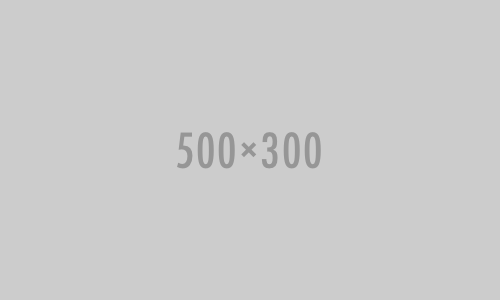
\includegraphics[width=0.5\textwidth]{./img/500X300.png}
\caption{The caption of the figure goes here.}
\label{fig:demo_figure_2}
\end{figure}

\par
Quis autem vel eum iure reprehenderit qui in ea voluptate velit esse quam nihil molestiae consequatur, vel illum qui dolorem eum fugiat quo voluptas nulla pariatur. Ut enim ad minima veniam, quis nostrum exercitationem ullam corporis suscipit laboriosam, nisi ut aliquid ex ea commodi consequatur? Quis autem vel eum iure reprehenderit qui in ea voluptate velit esse quam nihil molestiae consequatur, vel illum qui dolorem eum fugiat quo voluptas nulla pariatur.
% subsection subsection_112 (end)
% section section_11 (end)

\section{Section 2} % (fold)
\label{sec:section_12}
Quis autem vel eum iure reprehenderit qui in ea voluptate velit esse quam nihil molestiae consequatur, vel illum qui dolorem eum fugiat quo voluptas nulla pariatur. Ut enim ad minima veniam, quis nostrum exercitationem ullam corporis suscipit laboriosam, nisi ut aliquid ex ea commodi consequatur? Quis autem vel eum iure reprehenderit qui in ea voluptate velit esse quam nihil molestiae consequatur, vel illum qui dolorem eum fugiat quo voluptas nulla pariatur.

\par
Quis autem vel eum iure reprehenderit qui in ea voluptate velit esse quam nihil molestiae consequatur, vel illum qui dolorem eum fugiat quo voluptas nulla pariatur. Ut enim ad minima veniam, quis nostrum exercitationem ullam corporis suscipit laboriosam, nisi ut aliquid ex ea commodi consequatur? Quis autem vel eum iure reprehenderit qui in ea voluptate velit esse quam nihil molestiae consequatur, vel illum qui dolorem eum fugiat quo voluptas nulla pariatur.

\subsection{Subsection 1} % (fold)
\label{sub:subsection_121}
Quis autem vel eum iure reprehenderit qui in ea voluptate velit esse quam nihil molestiae consequatur, vel illum qui dolorem eum fugiat quo voluptas nulla pariatur. Ut enim ad minima veniam, quis nostrum exercitationem ullam corporis suscipit laboriosam, nisi ut aliquid ex ea commodi consequatur? Quis autem vel eum iure reprehenderit qui in ea voluptate velit esse quam nihil molestiae consequatur, vel illum qui dolorem eum fugiat quo voluptas nulla pariatur.

\par
Quis autem vel eum iure reprehenderit qui in ea voluptate velit esse quam nihil molestiae consequatur, vel illum qui dolorem eum fugiat quo voluptas nulla pariatur. Ut enim ad minima veniam, quis nostrum exercitationem ullam corporis suscipit laboriosam, nisi ut aliquid ex ea commodi consequatur? Quis autem vel eum iure reprehenderit qui in ea voluptate velit esse quam nihil molestiae consequatur, vel illum qui dolorem eum fugiat quo voluptas nulla pariatur.
% subsection subsection_121 (end)

\subsection{Subsection 2} % (fold)
\label{sub:subsection_122}
Quis autem vel eum iure reprehenderit qui in ea voluptate velit esse quam nihil molestiae consequatur, vel illum qui dolorem eum fugiat quo voluptas nulla pariatur. Ut enim ad minima veniam, quis nostrum exercitationem ullam corporis suscipit laboriosam, nisi ut aliquid ex ea commodi consequatur? Quis autem vel eum iure reprehenderit qui in ea voluptate velit esse quam nihil molestiae consequatur, vel illum qui dolorem eum fugiat quo voluptas nulla pariatur.

\par
Quis autem vel eum iure reprehenderit qui in ea voluptate velit esse quam nihil molestiae consequatur, vel illum qui dolorem eum fugiat quo voluptas nulla pariatur. Ut enim ad minima veniam, quis nostrum exercitationem ullam corporis suscipit laboriosam, nisi ut aliquid ex ea commodi consequatur? Quis autem vel eum iure reprehenderit qui in ea voluptate velit esse quam nihil molestiae consequatur, vel illum qui dolorem eum fugiat quo voluptas nulla pariatur.
% subsection subsection_122 (end)
% section section_12 (end)
    %!TEX root = ../thesis.tex
\chapter{Literature Review} % (fold)
\label{cha:_literature_review}

\section{Section 1} % (fold)
\label{sec:section_21}
Led ut perspiciatis unde omnis iste natus error sit voluptatem accusantium doloremque laudantium, totam rem aperiam, eaque ipsa quae ab illo inventore veritatis et quasi architecto beatae vitae dicta sunt explicabo. Nemo enim ipsam voluptatem quia voluptas sit aspernatur aut odit aut fugit, sed quia consequuntur magni dolores eos qui ratione voluptatem sequi nesciunt. Neque porro quisquam est, qui dolorem ipsum quia dolor sit amet, consectetur.

\par
Led ut perspiciatis unde omnis iste natus error sit voluptatem accusantium doloremque laudantium, totam rem aperiam, eaque ipsa quae ab illo inventore veritatis et quasi architecto beatae vitae dicta sunt explicabo. Nemo enim ipsam voluptatem quia voluptas sit aspernatur aut odit aut fugit, sed quia consequuntur magni dolores eos qui ratione voluptatem sequi nesciunt. Neque porro quisquam est, qui dolorem ipsum quia dolor sit amet, consectetur.

\subsection{Subsection 1} % (fold)
\label{sub:subsection_211}
Led ut perspiciatis unde omnis iste natus error sit voluptatem accusantium doloremque laudantium, totam rem aperiam, eaque ipsa quae ab illo inventore veritatis et quasi architecto beatae vitae dicta sunt explicabo. Nemo enim ipsam voluptatem quia voluptas sit aspernatur aut odit aut fugit, sed quia consequuntur magni dolores eos qui ratione voluptatem sequi nesciunt. Neque porro quisquam est, qui dolorem ipsum quia dolor sit amet, consectetur.

\begin{equation} \label{eq1}
  \begin{split}
    A & = \frac{\pi r^2}{2} \\
      & = \frac{1}{2} \pi r^2
  \end{split}
\end{equation}

\par
Adipisci velit, sed quia non numquam eius modi tempora incidunt ut labore et dolore magnam aliquam quaerat voluptatem. Ut enim ad minima veniam, quis nostrum exercitationem ullam corporis suscipit laboriosam, nisi ut aliquid ex ea commodi consequatur? Quis autem vel eum iure reprehenderit qui in ea voluptate velit esse quam nihil molestiae consequatur, vel illum qui dolorem eum fugiat quo voluptas nulla pariatur? \cite{bruno,smith}

\begin{table}[!htb]
\centering
    \begin{tabular}{abbb}
    \hline
    \rowcolor{Gray}
    \textsc{Column 1} & \textsc{Column 2} & \textsc{Column 3} & \textsc{Column 4}\\
    \hline
    1, 1 & 1, 2 & 1, 3 & 1, 4 \\
    2, 1 & 2, 2 & 2, 3 & 2, 4 \\
    3, 1 & 3, 2 & 3, 3 & 3, 4 \\
    4, 1 & 4, 2 & 4, 3 & 4, 4 \\ \hline
    \end{tabular}
    \caption{The caption of the table goes here.}
    \label{tab:demo_table}
\end{table}

\par
Lorem ipsum dolor sit amet, consectetur adipiscing elit, sed do eiusmod tempor incididunt ut labore et dolore magna aliqua. Ut enim ad minim veniam, quis nostrud exercitation ullamco\footnote{\label{foot_note_1}Led ut perspiciatis unde omnis iste natus error sit voluptatem accusantium doloremque laudantium, totam rem aperiam.} laboris nisi ut aliquip ex ea commodo consequat \cite{bruno}. Duis aute irure dolor in reprehenderit in voluptate velit esse cillum dolore eu fugiat nulla pariatur. Excepteur sint occaecat cupidatat non proident, sunt in culpa qui officia deserunt mollit anim id est laborum. \cite{smith}
\begin{multline}
p(x) = 3x^6 + 14x^5y + 590x^4y^2 + 19x^3y^3\\
- 12x^2y^4 - 12xy^5 + 2y^6 - a^3b^3
\end{multline}
% subsection subsection_211 (end)

\subsection{Subsection 2} % (fold)
\label{sub:subsection_212}
Led ut perspiciatis unde omnis iste natus error sit voluptatem accusantium doloremque laudantium, totam rem aperiam, eaque ipsa quae ab illo inventore veritatis et quasi architecto beatae vitae dicta sunt explicabo. Nemo enim ipsam voluptatem quia voluptas sit aspernatur aut odit aut fugit, sed quia consequuntur magni dolores eos qui ratione voluptatem sequi nesciunt. Neque porro quisquam est, qui dolorem ipsum quia dolor sit amet, consectetur.

\par
Led ut perspiciatis unde omnis iste natus error sit voluptatem accusantium doloremque laudantium, totam rem aperiam, eaque ipsa quae ab illo inventore veritatis et quasi architecto beatae vitae dicta sunt explicabo. Nemo enim ipsam voluptatem quia voluptas sit aspernatur aut odit aut fugit, sed quia consequuntur magni dolores eos qui ratione voluptatem sequi nesciunt. Neque porro quisquam est, qui dolorem ipsum quia dolor sit amet, consectetur.
% subsection subsection_212 (end)
% section section_21 (end)

\section{Section 2} % (fold)
\label{sec:section_22}
Led ut perspiciatis unde omnis iste natus error sit voluptatem accusantium doloremque laudantium, totam rem aperiam, eaque ipsa quae ab illo inventore veritatis et quasi architecto beatae vitae dicta sunt explicabo. Nemo enim ipsam voluptatem quia voluptas sit aspernatur aut odit aut fugit, sed quia consequuntur magni dolores eos qui ratione voluptatem sequi nesciunt. Neque porro quisquam est, qui dolorem ipsum quia dolor sit amet, consectetur.

\par
Led ut perspiciatis unde omnis iste natus error sit voluptatem accusantium doloremque laudantium, totam rem aperiam, eaque ipsa quae ab illo inventore veritatis et quasi architecto beatae vitae dicta sunt explicabo. Nemo enim ipsam voluptatem quia voluptas sit aspernatur aut odit aut fugit, sed quia consequuntur magni dolores eos qui ratione voluptatem sequi nesciunt. Neque porro quisquam est, qui dolorem ipsum quia dolor sit amet, consectetur.

\subsection{Subsection 1} % (fold)
\label{sub:subsection_221}
Led ut perspiciatis unde omnis iste natus error sit voluptatem accusantium doloremque laudantium, totam rem aperiam, eaque ipsa quae ab illo inventore veritatis et quasi architecto beatae vitae dicta sunt explicabo. Nemo enim ipsam voluptatem quia voluptas sit aspernatur aut odit aut fugit, sed quia consequuntur magni dolores eos qui ratione voluptatem sequi nesciunt. Neque porro quisquam est, qui dolorem ipsum quia dolor sit amet, consectetur.

\par
Led ut perspiciatis unde omnis iste natus error sit voluptatem accusantium doloremque laudantium, totam rem aperiam, eaque ipsa quae ab illo inventore veritatis et quasi architecto beatae vitae dicta sunt explicabo. Nemo enim ipsam voluptatem quia voluptas sit aspernatur aut odit aut fugit, sed quia consequuntur magni dolores eos qui ratione voluptatem sequi nesciunt. Neque porro quisquam est, qui dolorem ipsum quia dolor sit amet, consectetur.
% subsection subsection_221 (end)

\subsection{Subsection 2} % (fold)
\label{sub:subsection_222}
Led ut perspiciatis unde omnis iste natus error sit voluptatem accusantium doloremque laudantium, totam rem aperiam, eaque ipsa quae ab illo inventore veritatis et quasi architecto beatae vitae dicta sunt explicabo. Nemo enim ipsam voluptatem quia voluptas sit aspernatur aut odit aut fugit, sed quia consequuntur magni dolores eos qui ratione voluptatem sequi nesciunt. Neque porro quisquam est, qui dolorem ipsum quia dolor sit amet, consectetur.

\par
Led ut perspiciatis unde omnis iste natus error sit voluptatem accusantium doloremque laudantium, totam rem aperiam, eaque ipsa quae ab illo inventore veritatis et quasi architecto beatae vitae dicta sunt explicabo. Nemo enim ipsam voluptatem quia voluptas sit aspernatur aut odit aut fugit, sed quia consequuntur magni dolores eos qui ratione voluptatem sequi nesciunt. Neque porro quisquam est, qui dolorem ipsum quia dolor sit amet, consectetur.
% subsection subsection_222 (end)
% section section_22 (end)

    % \cleardoublepage
    \phantomsection
    \addcontentsline{toc}{chapter}{References}
    \bibliography{bibliography}
\end{document}